\section{Mission constraints}

The characteristic energy $C_3$ is a good estimator for the propulsion
requirements of a mission. If a propulsion system is imposed, its maximum
specific energy can be retrieved and imposed as a mission constraint to know
which targeting orbits can be followed.

Another mission constraint within the context of interlopers rendezvous is the
excess velocity at arrival. The faster the rendezvous, the greater the thrust
required for slowing down the spacecraft.

% Include a figure of the porkchop for oumumua
\newpage
\begin{figure}[H]
  \centering
  \includegraphics[width=\textwidth]{static/oumuamua/direct-transfer-porkchop.png}
  \caption{Porkchop plot for 1I/'Oumuamua}
  \label{fig:oumuamua-direct-transfer-porkchop}
\end{figure}

% Include a figure of the porkchop for oumumua
\newpage
\begin{figure}[H]
  \centering
  \includegraphics[width=\textwidth]{static/borisov/direct-transfer-porkchop.png}
  \caption{Porkchop plot for 2I/Borisov}
  \label{fig:borisov-direct-transfer-porkchop}
\end{figure}
